
%% bare_conf_compsoc.tex
%% V1.4b
%% 2015/08/26
%% by Michael Shell
%% See:
%% http://www.michaelshell.org/
%% for current contact information.
%%
%% This is a skeleton file demonstrating the use of IEEEtran.cls
%% (requires IEEEtran.cls version 1.8b or later) with an IEEE Computer
%% Society conference paper.
%%
%% Support sites:
%% http://www.michaelshell.org/tex/ieeetran/
%% http://www.ctan.org/pkg/ieeetran
%% and
%% http://www.ieee.org/

%%*************************************************************************
%% Legal Notice:
%% This code is offered as-is without any warranty either expressed or
%% implied; without even the implied warranty of MERCHANTABILITY or
%% FITNESS FOR A PARTICULAR PURPOSE! 
%% User assumes all risk.
%% In no event shall the IEEE or any contributor to this code be liable for
%% any damages or losses, including, but not limited to, incidental,
%% consequential, or any other damages, resulting from the use or misuse
%% of any information contained here.
%%
%% All comments are the opinions of their respective authors and are not
%% necessarily endorsed by the IEEE.
%%
%% This work is distributed under the LaTeX Project Public License (LPPL)
%% ( http://www.latex-project.org/ ) version 1.3, and may be freely used,
%% distributed and modified. A copy of the LPPL, version 1.3, is included
%% in the base LaTeX documentation of all distributions of LaTeX released
%% 2003/12/01 or later.
%% Retain all contribution notices and credits.
%% ** Modified files should be clearly indicated as such, including  **
%% ** renaming them and changing author support contact information. **
%%*************************************************************************


% *** Authors should verify (and, if needed, correct) their LaTeX system  ***
% *** with the testflow diagnostic prior to trusting their LaTeX platform ***
% *** with production work. The IEEE's font choices and paper sizes can   ***
% *** trigger bugs that do not appear when using other class files.       ***                          ***
% The testflow support page is at:
% http://www.michaelshell.org/tex/testflow/



\documentclass[conference,compsoc]{IEEEtran}
% Some/most Computer Society conferences require the compsoc mode option,
% but others may want the standard conference format.
%
% If IEEEtran.cls has not been installed into the LaTeX system files,
% manually specify the path to it like:
% \documentclass[conference,compsoc]{../sty/IEEEtran}





% Some very useful LaTeX packages include:
% (uncomment the ones you want to load)


% *** MISC UTILITY PACKAGES ***
%
%\usepackage{ifpdf}
% Heiko Oberdiek's ifpdf.sty is very useful if you need conditional
% compilation based on whether the output is pdf or dvi.
% usage:
% \ifpdf
%   % pdf code
% \else
%   % dvi code
% \fi
% The latest version of ifpdf.sty can be obtained from:
% http://www.ctan.org/pkg/ifpdf
% Also, note that IEEEtran.cls V1.7 and later provides a builtin
% \ifCLASSINFOpdf conditional that works the same way.
% When switching from latex to pdflatex and vice-versa, the compiler may
% have to be run twice to clear warning/error messages.


% *** LANGUAGE PACKAGES ***
\usepackage{german}
\usepackage[UTF8]{inputenc}
\usepackage[T1]{fontenc} %für Umlautdarstellung



% *** CITATION PACKAGES ***
%
\ifCLASSOPTIONcompsoc
  % IEEE Computer Society needs nocompress option
  % requires cite.sty v4.0 or later (November 2003)
  \usepackage[nocompress]{cite}
\else
  % normal IEEE
  \usepackage{cite}
\fi
\usepackage{csquotes}
% cite.sty was written by Donald Arseneau
% V1.6 and later of IEEEtran pre-defines the format of the cite.sty package
% \cite{} output to follow that of the IEEE. Loading the cite package will
% result in citation numbers being automatically sorted and properly
% "compressed/ranged". e.g., [1], [9], [2], [7], [5], [6] without using
% cite.sty will become [1], [2], [5]--[7], [9] using cite.sty. cite.sty's
% \cite will automatically add leading space, if needed. Use cite.sty's
% noadjust option (cite.sty V3.8 and later) if you want to turn this off
% such as if a citation ever needs to be enclosed in parenthesis.
% cite.sty is already installed on most LaTeX systems. Be sure and use
% version 5.0 (2009-03-20) and later if using hyperref.sty.
% The latest version can be obtained at:
% http://www.ctan.org/pkg/cite
% The documentation is contained in the cite.sty file itself.
%
% Note that some packages require special options to format as the Computer
% Society requires. In particular, Computer Society  papers do not use
% compressed citation ranges as is done in typical IEEE papers
% (e.g., [1]-[4]). Instead, they list every citation separately in order
% (e.g., [1], [2], [3], [4]). To get the latter we need to load the cite
% package with the nocompress option which is supported by cite.sty v4.0
% and later.





% *** GRAPHICS RELATED PACKAGES ***
%
\ifCLASSINFOpdf
   \usepackage[pdftex]{graphicx}
  % declare the path(s) where your graphic files are
  % \graphicspath{{../pdf/}{../jpeg/}}
  % and their extensions so you won't have to specify these with
  % every instance of \includegraphics
  %\DeclareGraphicsExtensions{.pdf,.jpeg,.png}
\else
  % or other class option (dvipsone, dvipdf, if not using dvips). graphicx
  % will default to the driver specified in the system graphics.cfg if no
  % driver is specified.
  % \usepackage[dvips]{graphicx}
  % declare the path(s) where your graphic files are
  % \graphicspath{{../eps/}}
  % and their extensions so you won't have to specify these with
  % every instance of \includegraphics
  % \DeclareGraphicsExtensions{.eps}
\fi
% graphicx was written by David Carlisle and Sebastian Rahtz. It is
% required if you want graphics, photos, etc. graphicx.sty is already
% installed on most LaTeX systems. The latest version and documentation
% can be obtained at: 
% http://www.ctan.org/pkg/graphicx
% Another good source of documentation is üsing Imported Graphics in
% LaTeX2e" by Keith Reckdahl which can be found at:
% http://www.ctan.org/pkg/epslatex
%
% latex, and pdflatex in dvi mode, support graphics in encapsulated
% postscript (.eps) format. pdflatex in pdf mode supports graphics
% in .pdf, .jpeg, .png and .mps (metapost) formats. Users should ensure
% that all non-photo figures use a vector format (.eps, .pdf, .mps) and
% not a bitmapped formats (.jpeg, .png). The IEEE frowns on bitmapped formats
% which can result in "jaggedy"/blurry rendering of lines and letters as
% well as large increases in file sizes.
%
% You can find documentation about the pdfTeX application at:
% http://www.tug.org/applications/pdftex





% *** MATH PACKAGES ***
%
%\usepackage{amsmath}
% A popular package from the American Mathematical Society that provides
% many useful and powerful commands for dealing with mathematics.
%
% Note that the amsmath package sets \interdisplaylinepenalty to 10000
% thus preventing page breaks from occurring within multiline equations. Use:
%\interdisplaylinepenalty=2500
% after loading amsmath to restore such page breaks as IEEEtran.cls normally
% does. amsmath.sty is already installed on most LaTeX systems. The latest
% version and documentation can be obtained at:
% http://www.ctan.org/pkg/amsmath





% *** SPECIALIZED LIST PACKAGES ***
%
%\usepackage{algorithmic}
% algorithmic.sty was written by Peter Williams and Rogerio Brito.
% This package provides an algorithmic environment fo describing algorithms.
% You can use the algorithmic environment in-text or within a figure
% environment to provide for a floating algorithm. Do NOT use the algorithm
% floating environment provided by algorithm.sty (by the same authors) or
% algorithm2e.sty (by Christophe Fiorio) as the IEEE does not use dedicated
% algorithm float types and packages that provide these will not provide
% correct IEEE style captions. The latest version and documentation of
% algorithmic.sty can be obtained at:
% http://www.ctan.org/pkg/algorithms
% Also of interest may be the (relatively newer and more customizable)
% algorithmicx.sty package by Szasz Janos:
% http://www.ctan.org/pkg/algorithmicx




% *** ALIGNMENT PACKAGES ***
%
%\usepackage{array}
% Frank Mittelbach's and David Carlisle's array.sty patches and improves
% the standard LaTeX2e array and tabular environments to provide better
% appearance and additional user controls. As the default LaTeX2e table
% generation code is lacking to the point of almost being broken with
% respect to the quality of the end results, all users are strongly
% advised to use an enhanced (at the very least that provided by array.sty)
% set of table tools. array.sty is already installed on most systems. The
% latest version and documentation can be obtained at:
% http://www.ctan.org/pkg/array


% IEEEtran contains the IEEEeqnarray family of commands that can be used to
% generate multiline equations as well as matrices, tables, etc., of high
% quality.




% *** SUBFIGURE PACKAGES ***
%\ifCLASSOPTIONcompsoc
%  \usepackage[caption=false,font=footnotesize,labelfont=sf,textfont=sf]{subfig}
%\else
%  \usepackage[caption=false,font=footnotesize]{subfig}
%\fi
% subfig.sty, written by Steven Douglas Cochran, is the modern replacement
% for subfigure.sty, the latter of which is no longer maintained and is
% incompatible with some LaTeX packages including fixltx2e. However,
% subfig.sty requires and automatically loads Axel Sommerfeldt's caption.sty
% which will override IEEEtran.cls' handling of captions and this will result
% in non-IEEE style figure/table captions. To prevent this problem, be sure
% and invoke subfig.sty's "caption=false" package option (available since
% subfig.sty version 1.3, 2005/06/28) as this is will preserve IEEEtran.cls
% handling of captions.
% Note that the Computer Society format requires a sans serif font rather
% than the serif font used in traditional IEEE formatting and thus the need
% to invoke different subfig.sty package options depending on whether
% compsoc mode has been enabled.
%
% The latest version and documentation of subfig.sty can be obtained at:
% http://www.ctan.org/pkg/subfig




% *** FLOAT PACKAGES ***
%
%\usepackage{fixltx2e}
% fixltx2e, the successor to the earlier fix2col.sty, was written by
% Frank Mittelbach and David Carlisle. This package corrects a few problems
% in the LaTeX2e kernel, the most notable of which is that in current
% LaTeX2e releases, the ordering of single and double column floats is not
% guaranteed to be preserved. Thus, an unpatched LaTeX2e can allow a
% single column figure to be placed prior to an earlier double column
% figure.
% Be aware that LaTeX2e kernels dated 2015 and later have fixltx2e.sty's
% corrections already built into the system in which case a warning will
% be issued if an attempt is made to load fixltx2e.sty as it is no longer
% needed.
% The latest version and documentation can be found at:
% http://www.ctan.org/pkg/fixltx2e


%\usepackage{stfloats}
% stfloats.sty was written by Sigitas Tolusis. This package gives LaTeX2e
% the ability to do double column floats at the bottom of the page as well
% as the top. (e.g., "\begin{figure*}[!b]" is not normally possible in
% LaTeX2e). It also provides a command:
%\fnbelowfloat
% to enable the placement of footnotes below bottom floats (the standard
% LaTeX2e kernel puts them above bottom floats). This is an invasive package
% which rewrites many portions of the LaTeX2e float routines. It may not work
% with other packages that modify the LaTeX2e float routines. The latest
% version and documentation can be obtained at:
% http://www.ctan.org/pkg/stfloats
% Do not use the stfloats baselinefloat ability as the IEEE does not allow
% \baselineskip to stretch. Authors submitting work to the IEEE should note
% that the IEEE rarely uses double column equations and that authors should try
% to avoid such use. Do not be tempted to use the cuted.sty or midfloat.sty
% packages (also by Sigitas Tolusis) as the IEEE does not format its papers in
% such ways.
% Do not attempt to use stfloats with fixltx2e as they are incompatible.
% Instead, use Morten Hogholm'a dblfloatfix which combines the features
% of both fixltx2e and stfloats:
%
% \usepackage{dblfloatfix}
% The latest version can be found at:
% http://www.ctan.org/pkg/dblfloatfix




% *** PDF, URL AND HYPERLINK PACKAGES ***
%
%\usepackage{url}
% url.sty was written by Donald Arseneau. It provides better support for
% handling and breaking URLs. url.sty is already installed on most LaTeX
% systems. The latest version and documentation can be obtained at:
% http://www.ctan.org/pkg/url
% Basically, \url{my_url_here}.




% *** Do not adjust lengths that control margins, column widths, etc. ***
% *** Do not use packages that alter fonts (such as pslatex).         ***
% There should be no need to do such things with IEEEtran.cls V1.6 and later.
% (Unless specifically asked to do so by the journal or conference you plan
% to submit to, of course. )


% correct bad hyphenation here
\hyphenation{op-tical net-works semi-conduc-tor}


\begin{document}
%
% paper title
% Titles are generally capitalized except for words such as a, an, and, as,
% at, but, by, for, in, nor, of, on, or, the, to and up, which are usually
% not capitalized unless they are the first or last word of the title.
% Linebreaks \\ can be used within to get better formatting as desired.
% Do not put math or special symbols in the title.
\title{Service Discovery im Internet of Things}


% author names and affiliations
% use a multiple column layout for up to three different
% affiliations
\author{
\IEEEauthorblockN{Merlin Gernsheimer}
\IEEEauthorblockA{Hochschule Furtwangen University\\
Furtwangen, Deutschland\\
Email: merlin.gernsheimer@hs-furtwangen.de}
\and
\IEEEauthorblockN{Peter Wursthorn}
\IEEEauthorblockA{Hochschule Furtwangen University\\
Furtwangen, Deutschland\\
Email: peter.wursthorn@hs-furtwangen.de}}

% conference papers do not typically use \thanks and this command
% is locked out in conference mode. If really needed, such as for
% the acknowledgment of grants, issue a \IEEEoverridecommandlockouts
% after \documentclass

% for over three affiliations, or if they all won't fit within the width
% of the page (and note that there is less available width in this regard for
% compsoc conferences compared to traditional conferences), use this
% alternative format:
% 
%\author{\IEEEauthorblockN{Michael Shell\IEEEauthorrefmark{1},
%Homer Simpson\IEEEauthorrefmark{2},
%James Kirk\IEEEauthorrefmark{3}, 
%Montgomery Scott\IEEEauthorrefmark{3} and
%Eldon Tyrell\IEEEauthorrefmark{4}}
%\IEEEauthorblockA{\IEEEauthorrefmark{1}School of Electrical and Computer Engineering\\
%Georgia Institute of Technology,
%Atlanta, Georgia 30332--0250\\ Email: see http://www.michaelshell.org/contact.html}
%\IEEEauthorblockA{\IEEEauthorrefmark{2}Twentieth Century Fox, Springfield, USA\\
%Email: homer@thesimpsons.com}
%\IEEEauthorblockA{\IEEEauthorrefmark{3}Starfleet Academy, San Francisco, California 96678-2391\\
%Telephone: (800) 555--1212, Fax: (888) 555--1212}
%\IEEEauthorblockA{\IEEEauthorrefmark{4}Tyrell Inc., 123 Replicant Street, Los Angeles, California 90210--4321}}




% use for special paper notices
%\IEEEspecialpapernotice{(Invited Paper)}




% make the title area
\maketitle

% As a general rule, do not put math, special symbols or citations
% in the abstract
\begin{abstract}
The abstract goes here.
\end{abstract}

% no keywords




% For peer review papers, you can put extra information on the cover
% page as needed:
% \ifCLASSOPTIONpeerreview
% \begin{center} \bfseries EDICS Category: 3-BBND \end{center}
% \fi
%
% For peerreview papers, this IEEEtran command inserts a page break and
% creates the second title. It will be ignored for other modes.
\IEEEpeerreviewmaketitle



\section{Einführung}
Das Internet der Dinge (engl. Internet of Things/IoT) nimmt einen immer größeren Stellenwert ein, da es beständig wächst. Neben klassischen internetfähigen Geräten wie Desktop-Computern oder Smartphones sind heutzutage viele Geräte mit dem World Wide Web verbunden, die keine traditionellen Teilnehmer des Internets sind. Manche Geräte, wie Beispiel Sensoren für wissenschaftliche Untersuchungen liefern dabei nur Daten. Andere Geräte hingegen sind über das Internet steuerbar.
Gerade die Entwicklung des Smart-Home-Konzeptes hat die Anzahl der Geräte letzter Art befeuert. Von der Steckdose bis zur Klimaanlage stehen dem Verbraucher Modelle zur Verfügung, die an das Internet angeschlossen sind und bequem von überall gesteuert werden können.

Die Vielzahl dieser Geräte wirft eine entscheidende Frage auf: Wie können bei so einer Vielzahl an Geräten die richtigen Geräte gefunden werden?

Im weiteren Verlauf dieser Arbeit setzen wir uns zunächst mit diversen Frameworks auseinander, die das Auffinden von IoT-Geräten erleichtern oder komplett übernehmen. Anschließend werden diese Frameworks anhand mehrerer Kriterien untersucht, um herauszufinden, welches sich am besten für die zukünftige Weiterentwicklung der Entdeckung von IoT-Geräten eignet.

\section{Frameworks}
Um die Entdeckung von IoT Geräten von der bisher bekannten Entdeckung von \enquote{normalen} Services abzugrenzen werden folgen verschiedene Frameworks vorgestellt, die sich mit der Entdeckung von Services auseinandersetzen, aufgrund dieser Beschreibungen kann dann im folgenden Kapitel ein Vergleich von IoT-Discovery mit herkömmlicher Service Discovery gezogen werden.

\subsection{Simurgh}

Simurgh ist ein Framework, das versucht, das Design und die Wiederverwendbarkeit von IoT-Anwendungen zu erleichtern und die Verwaltung eines IoT basierten Systems zu vereinfachen. Dies wird  durch eine schichtenbasiert zunehmende Abstraktion von Geräten und ihrer Funktionsweise gegenüber der nutzenden Schicht realisiert. Diese Schichten lassen sich in zwei Gruppen unterteilen, eine \enquote{Things} Schicht und eine \enquote{Platform} Schicht. (vgl. \cite{simurgh})

Die Platform Schicht übernimmt hierbei die Interaktion mit einem eventuellen Nutzer, diesem werden sog. \enquote{Flows} zur Verfügung gestellt. Durch die Verkettung und Konfiguration dieser \enquote{Flows} kann der Nutzer ein für seine Anforderungen spezifisch erstelltes Programm in Bearbeitung geben, das benötigte Daten von der \enquote{Things} Schicht automatisch anfordert. Um diese Datenanforderung zuverlässig gewährleisten zu können hält sich die Platform Schicht Beschreibungen der ihr bekannten Geräte vor, über welche ein, bzw. mehrere zu der Anfrage passende Geräte gefunden werden. Diese Beschreibungen werden nicht direkt von den Geräten erwartet, sondern von der \enquote{Things} Schicht bereitgestellt. Die Beschreibungen sind hierbei in zwei Teile aufgeteilt, zum einen ein sog. \enquote{Thing Description Document(TDD)} welches eine allgemeine Beschreibung des Geräts und seines Besitzers beinhaltet und zum andren Verweise auf Dokumente, welche die APIs des Geräts beschreiben. Standardmäßig unterstützt das Framework die Beschreibungssprache \enquote{RESTful API Modeling Language(RAML)}, welche weit weniger verbos als z.B. eine entsprechende Beschreibung in der XML-basierten Web Service Description Language ist. (vgl. \cite{simurgh})

Die \enquote{Things} Schicht setzt sich direkt mit den verschiedenen Geräten auseinander. Die Things Schicht repräsentiert hier eine zentralisierte Verwaltung von Geräten, die Schnittstellen für die \enquote{Platform} Schicht zur Verfügung stellt. Sie verlässt sich hierbei darauf, dass Geräte sich selbstständig einer sog. Domain anschließen und Informationen bereitgestellt werden, aus welchen die Beschreibung für die Platform Schicht generiert werden kann. (vgl. \cite{simurgh})

Um die Kommunikation mit der Platform Schicht zu vereinfachen, werden die meist hersteller-, protokoll- und/oder sprachspezifischen APIs der einzelnen Geräte von der Things Schicht abstrahiert und in einem einheitlichen Stil ansprechbar gemacht. Hierzu verfügt die Things Schicht über Bibliotheken, die allerdings für Integration eines neuen Gerätetyps erstellt und darauffolgend gewartet werden muss, was die Anwendbarkeit des Frameworks beeinflusst. (vgl. \cite{simurgh}) 

\subsection{Discovery-Driven Service Oriented Architecture}
Der folgende Architekturvorschlag für entdeckungsbasierte Service-Orientierung wurde leider bis jetzt noch mit keinem kürzerem Namen versehen. Deshalb wird er im weiteren Verlauf mit DDSO abgekürzt.

DDSP betrachtet Discovery von Geräten ein einem breiteren Spektrum als nur zur direkten Abfrage von Daten. Es versucht, IoT-Geräte in ein Cloud-basiertes Umfeld von Applikationen und Services einzuordnen. Hierzu wird eine Anwendung, die das IoT nutzt, in drei Funktionalitätsbereichen modelliert, die je nach Anwendung verschieden stark verwendet werden. (vgl. \cite{DDSO}) Diese Bereiche sind folgende:

\begin{itemize}
\item \textbf{Devices} Setzt sich direkt mit zentralisierter Kommunikation mit und  Verwaltung von Geräten auseinander
\item \textbf{Data} Repräsentiert Datenhaltungssysteme um Ergebnisse der anderen Bereiche transparent speichern und abrufen zu können
\item \textbf{Application} Repräsentiert verschiedene Applikationen und Services, die sowohl von Endnutzern als auch gegenseitig aufrufbar sind.
\end{itemize}

In jedem der drei Funktionalitätsbereiche, sowie zwischen allen drei findet außerdem dauerhaft eine automatische Discovery, Integration und Repräsentation von Geräten, Services und Daten statt. Dieser Prozess sorgt dafür, dass auch bereichsintern immer mit den neuesten Informationen zu vorhandenen Geräten/Services/Daten gearbeitet wird. Weiterhin sorgt dieser Mechanismus dafür, dass auch bei Ausfällen innerhalb eines Bereichs schnell ein Ersatz gefunden werden kann. (vgl. \cite{DDSO})

DDSO soll als eine Erweiterung des \enquote{OpenIoT} Frameworks eingesetzt werden, welches sich bis jetzt nur mit der Discorvery von Geräten auseinandersetzt. Der \enquote{Devices} Bereich der DDSO Architektur soll durch die bis jetzt vorhandenen Funktionalitäten von OpenIoT abgedeckt werden. Die anderen Bereiche des vorgeschlagenen Modells kann OpenIoT allerdings noch nicht bedienen. (vgl. \cite{DDSO})

\subsection{Efficient semantic-based IoT service discovery}

Der Ansatz dieses Mechanismus ist die Einführung von semantischen Gateways, die in einer hierarchischen Struktur aufgebaut sind. Im Kern soll es damit ermöglicht werden, in einem dynamischen Kontext die effiziente Suche nach Webservices zu ermöglichen. (vgl. \cite{efficientSemantic})

Die Hierarchie der semantischen Gateways wird bestimmt durch sogenannte Smart Spaces. Diese Smart Spaces repräsentieren unterschiedlich große räumliche Gebiete, beispielsweise ein Land, eine Region, eine Stadt, eine Straße, ein Haus oder auch nur ein einzelner Raum. Dabei wird jeder Smart Space durch ein semantisches Gateway gekapselt. (vgl. \cite{efficientSemantic})

Das semantische Gateway selbst ist eine Softwarekomponente, die Informationen über in ihrem Bereich liegende IoT-Services verwaltet. Zusätzlich nimmt ein Gateway Service-Discovery-Anfragen entgegen und vermittelt eine Anfrage an einen Service, der die gesuchten Kriterien erfüllt. Im Inneren besteht ein semantisches Gateway aus mehreren Knoten. Dabei wird zwischen High-Level-Knoten und Low-Level-Knoten unterschieden. (vgl. \cite{efficientSemantic})

Low-Level-Knoten verwalten die Beschreibungen der Services, die an dem betreffenden Gateway registriert sind. Die High-Level-Knoten wiederum verwalten die Informationen, die benutzt werden um die Verbindung zwischen einer Anfrage und einem Service herzustellen und bilden somit das Kernstück der Funktionalität. (vgl. \cite{efficientSemantic})

Im speziellen werden die dem Gateway bekannten Services in unterschiedliche Cluster unterteilt. Die Zuteilung zu einem Cluster erfolgt je nach dem Aufgabengebiet, das ein Service bearbeitet. Somit werden Services gleicher Funktionalität gesammelt. Dies dient dazu, bei einer Anfrage mit möglichst geringen Kosten den richtigen Service vermitteln zu können. (vgl. \cite{efficientSemantic})

Die Kosten geben die Autoren als Anzahl der Operationen an, die ausgeführt werden müssen, um innerhalb eines Gateways einen Service zu finden, der die Anfrage zufriedenstellend erfüllt. Die Bildung von semantischen Clustern führt dazu, dass das System mit der Zeit optimiert wird und die Kosten einer Service-Discovery-Anfrage somit sinken, je mehr Services dem Gateway bekannt sind. (vgl. \cite{efficientSemantic})

Wenn die nach der Registrierung eines Service erfolgende Aggregation der Daten abgeschlossen ist, werden diese Daten dem Eltern-Gateway übermittelt, welches sie einerseits speichert, andererseits seinem eigenen Eltern-Gateway weiterreicht, bis die neuen Informationen schließlich das Gateway an der Spitze der Hierarchie erreichen. Auf diese Weise wird es ermöglicht, dass jede Hierarchie den Überblick über registrierte Services der tieferliegenden Hierarchieebenen hat und somit eingehende Anfragen optimal vermitteln kann. (vgl. \cite{efficientSemantic})

\subsection{An Energy-Efficient Service Discovery Protocol}

Problematisch an dem im vorhergehenden Absatz erläuterten Mechanismus ist, dass die verwendeten Gateways sogenannte Single-Point-of-Failures darstellen, d.h. Punkte, die kritisch für die Ausführung des Systems sind, respektive bei deren Nicht-Verfügbarkeit das gesamte System lahmgelegt wird. Zusätzlich wird auch darauf hingewiesen, dass bei einer realistischen Anzahl an IoT-Geräten (~Milliarden) die Anzahl der benötigten Gateways unrealistisch stark ansteigen würde. Deshalb verfolgt das in diesem Abschnitt vorgestellte Protokoll einen dezentralisierten Ansatz, der die Ausfallsicherheit erhöht. (vgl. \cite{energy-efficient})

\begin{figure}
\centering
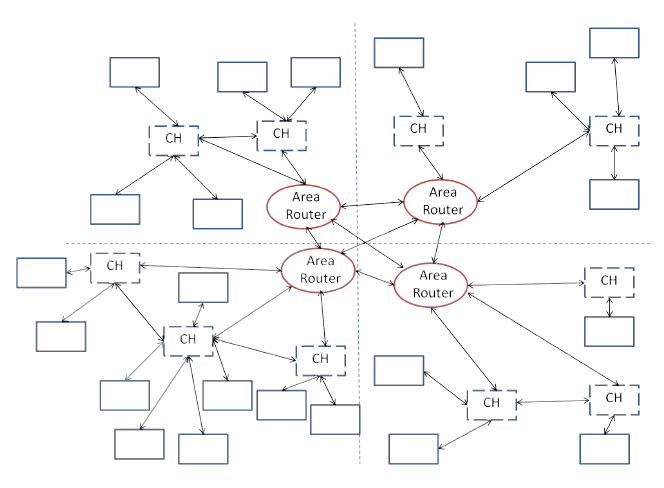
\includegraphics[scale=0.45]{EEP.png}
\caption{EEP Übersicht}
\label{EEPBild}
Quelle: \cite{energy-efficient}
\end{figure}

Da IoT-Geräte eine sehr hohe Diversität aufweisen, fokussiert sich der Ansatz zunächst nur darauf, mit einem Smartphone verschiedenste Sensoren in der erweiterten Umgebung zu finden. Dabei wird bewusst nur ein Ansatz zur Verbindung mit lokalen Services gewählt, da dieser Ansatz erst zu einem späteren Zeitpunkt auf die globale Ebene ausgeweitet werden soll. Bei der Suche eines Smartphones nach einem Service, der bestimmte Sensordaten zur Verfügung stellt, wird bei der Anfrage eine Liste von Kriterien gesendet, die ein Service erfüllen soll. (vgl. \cite{energy-efficient})

Die Vermittlung der Anfrage an den passenden Service erfolgt durch eine dreischichtige Architektur. Kernpunkt der Architektur bilden sogenannte Cluster Heads, die Informationen über Services in ihrer direkten Nähe speichern. Diese Cluster Heads werden an zufälligen Punkten erstellt. Wenn ein Cluster Head ausfallen sollte, kann die Anfrage einfach von einem anderen bearbeitet werden, was zu einer erhöhten Verfügbarkeit gegenüber einem Ansatz über Gateways führt. (vgl. \cite{energy-efficient})

Sofern ein Cluster Head eine Anfrage nicht zufriedenstellend an einen Service vermitteln kann, wird die Anfrage stattdessen an die oberste Schicht der Architektur weitergeleitet, den sogenannten Area Router. Der Area Router ist mit allen Cluster Heads eines abgegrenzten räumlichen Bereiches verbunden und speichert Informationen über die dort bekannten Services. Fall ein Cluster Head unter den Service in seiner direkten Umgebung keinen zu einer Anfrage passenden Service findet, kann der Area Router einspringen, da er wesentlich mehr Services kennt. Zusätzlich ist es möglich, das abgedeckte Gebiet zu erweitern, in dem mehrere Area Router zusammengeschaltet werden. (vgl. \cite{energy-efficient})

Dadurch, dass die Suche nach passenden Services erst in der unmittelbaren Umgebung erfolgt und nur ausgeweitet wird, falls keine Ergebnisse gefunden werden, wird Energie gespart. Zusätzlich prüft der Mechanismus regelmäßig, ob und wie häufig Cluster Heads angesprochen werden. Wird bei dieser Prüfung festgestellt, dass ein Cluster Head nur sehr selten Anfragen bekommt und aktiv werden muss, so wird er in den Sleep-Modus versetzt, wodurch zusätzlich die Energieeffizienz gesteigert wird. (vgl. \cite{energy-efficient})

\subsection{UDDI}

Universal Description, Discovery and Integration (UDDI) ist ein standardisierter Verzeichnisdienst, mit dessen Hilfe Anfragen zwischen Clients und Webservices vermittelt werden sollen. Entwickelt und vorangetrieben wurde UDDI als gemeinsames Projekt von IBM, Microsoft und SAP. Ende 2005 schalteten diese Firmen jedoch ihre UDDI-Technologien ab. (vgl. \cite{UDDI-Variability})

Laut \cite{UDDI-Variability} war UDDI in der Version 1.0 nicht zuverlässig, da die Spezifikation in vielen Punkten zu ungenau formuliert war, um als Industriestandard zu genügen. Wohl auch deshalb fand UDDI anfangs eine wesentlich geringere Akzeptanz als erwartet. Mit der Version 2.0 wurde die Spezifikation im Mai 2003 an vielen Punkten verbessert, so dass diese Version als erste zuverlässige Version angesehen wird.

Der Prozess der UDDI-Technologie besteht aus drei Schritten:
\begin{itemize}
\item[1.] Veröffentlichen eines Service (durch den Service-Anbieter)
\item[2.] Suche eines Clients nach einem Service, welcher bestimmte Kriterien erfüllt
\item[3.] Verbindung eines Clients zu dem in der UDDI-Registry gefundenen Service
\end{itemize}

Konkrete Implementationen von UDDI können entweder global oder lokal ausgelegt sein. Das heißt, es ist einerseits möglich, mit einer UDDI-Implementation die registrierten Services über das Internet jedem beliebigen Client zur Verfügung zu stellen (global) oder andererseits, die Services nur innerhalb eines begrenzten Computernetzes anzubieten. Letzteres ist besonders für Unternehmen interessant, da Webservices in deren Kontext oftmals Geschäftslogik enthalten.

Die Informationen über einen an einem UDDI-Dienst registrierte Service werden in drei Kategorien unterteilt. Diese werden angelehnt an das Farbschema von Telefonbüchern als Weiße, Gelbe und Grüne Seiten bezeichnet. Die weißen Seiten beinhalten dabei Informationen über den Anbieter und sein Geschäftsfeld. Diese grundlegenden Informationen umfassen beispielsweise Kontaktinformationen wie Adresse, Telefonnummer und den Namen. Zudem wird dem Anbieter eine einzigartige ID zugeordnet, über die er identifiziert werden kann. (vgl. \cite{UDDI-implementation})

Die Gelben Seiten enthalten somit weitergehende Informationen über den Anbieter und beschreiben dabei seine technologischen Kompetenzen, damit eventuell an einem seiner Services interessierte Clients den Anbieter einschätzen können. Dies kann gleichzeitig dazu genutzt werden, um die registrierten Anbieter und Services nach bestimmten Geschäftsfeldern zu durchsuchen. (vgl. \cite{UDDI-implementation})

Als letztes enthalten die Grünen Seiten die eigentlichen technischen Informationen zu einem Service. Diese technischen Informationen umfassen zum einen die vorhandenen Schnittstellen und URL-Adressen, sowie auch die Discovery-Informationen, die benötigt werden um die Verbindung zu einem Service herzustellen. (vgl. \cite{UDDI-implementation})

\section{Bewertung}

\subsection{Scope}

Bei der Bewertung einer Technologie für Service-Discovery spielen die Scopes, in deren Kontext die Service-Discovery stattfindet eine große Rolle. Dabei muss zwischen zwei Arten von Scopes unterschieden werden.
Der erste Scope, dessen Auswahl entscheidend für die Bewertung der Technologie ist, ist die Reichweite, innerhalb derer Services gesucht werden sollen. Dabei wird unterschieden zwischen einem globalen Scope und einem lokalen Scope. Global bedeutet, dass Services im Kontext des gesamten Internets verwaltet werden, während lokale Ansätze zur Service-Discovery nur ein begrenztes Computernetz variabler Größe verwalten. Rückblickend betrachtet war die Entscheidung, UDDI hauptsächlich als internetweiten (also globalen) Dienst für die Registrierung von Services voranzutreiben einer der größten Fehler hinsichtlich der Entwicklung dieser Technologie. Angetrieben durch den üblichen Hype-Cycle bei der Entwicklung neuer Software-Technologien wurde fälschlicherweise angenommen, dass Anbieter wie Anwender die Nutzung eines zentralen Registrierungsdienstes favorisieren würden.

Wie die Realität gezeigt hat, scheuen sich insbesondere die Anbieter von Webservices, ihre Dienste frei zur Verfügung zu stellen. Gerade Firmen, deren Services oftmals Geschäftslogik enthalten, bevorzugen eine lokale Lösung zur Service-Discovery, bei der ihre Services nur innerhalb des Firmennetzes verfügbar gemacht werden. Diese Entwicklung spiegeln auch die in dieser Arbeit vorgestellten Ansätze wieder, die hauptsächlich lokale Implementierungen fokussieren.

Gerade im Internet der Dinge kommt lokalen Ansätzen eine tragende Rolle zu. Smart-Home verbindet eine große Menge an Geräten mit dem Internet, deren Services deutlich beschränkter sind als die klassischen Webservices. Diese Geräte, die meist über eine REST-Schnittstelle angesprochen werden können, sollen nur im Scope des jeweiligen Hauses gefunden und angesprochen werden können. Der korrekte Scope ist hier von Bedeutung, da eine Entblößung in einem größeren Kontext ein mögliches Sicherheitsproblem darstellt.

Der zweite maßgebliche Scope ist die Art der IoT-Geräte, die durch die Service-Discovery-Technologie verwaltet werden sollen. Wie vorhergehend erwähnt, verzeichnen gerade Smart-Home-Geräte einen starken Anstieg bei der Verbreitung. Dabei werden alle möglichen Haushaltsgeräte an das Internet angeschlossen, um diese zentral steuern zu können. Derartige Geräte umfassen alles angefangen von intelligenten Steckdosen über intelligente Küchengeräte bis hin zu intelligenten Beleuchtungs- und Heizsystemen. Bei dieser Art von Gerät spielt in der Regel die Fernsteuerung eines physischen Gerätes die Hauptrolle, das heißt der Fokus liegt auf dem Senden von Daten. Einen ganz anderen Scope stellen beispielsweise Sensoren für wissenschaftliche Untersuchungen dar, also zum Beispiel Luftdruck oder Temperatursensoren. Aufgrund der hohen Diversität der Geräte konzentrieren sich Technologien für die Service-Discovery meist auf einen bestimmten Typ von Gerät. Da es sich bei den meisten, von IoT-Geräten angebotenen, Services nur um rudimentäre Services ohne detaillierte Beschreibungen wie WSDL-Dokumente handelt, können nur bedingt Aussagen über die jeweiligen Services getroffen werden, sodass es sich anbietet, von vorneherein nur Services mit einer semantischen Ähnlichkeit zu verwalten.

Zusammengefasst lässt sich also sagen, dass hinsichtlich des Scopes bei der Service-Discovery für das Internet der Dinge eine Einschränkung der verwalteten Geräte sowohl in Bezug auf die Größe des verwalteten Bereiches als auch auf die Art des angebotenen Service sinnvoll ist.

\subsection{Hardware} \label{Hardware}

Die Hardware unterscheidet sich bei Services im Internet der Dinge massiv von der Hardware normaler Webservices. Während letztere in der Regel mit der nötigen Hardware ausgestattet sind, die es braucht um eine breite Geschäftslogik abzuarbeiten, sind IoT-Services mit sehr viel schwächerer Hardware ausgestattet. Zudem kommt die zuvor erwähnte Problematik, dass bei dieser Art von Services meist ein beschreibendes Dokument fehlt und somit nicht ohne weiteres Aussagen über die semantische Bedeutung eines Service getroffen werden können.

Grundsätzlich gibt es zwei mögliche Ansätze um Service-Discovery durchzuführen. Einerseits ist es möglich, zentrale Komponenten für die Registrierung von Services zu schaffen, andererseits kann innerhalb eines Netzwerkes per Broadcast nach Services gesucht werden, womit die Suche dezentral funktioniert. Die vorgestellten Ansätze verfolgen ausnahmslos den ersteren, zentralistischen Ansatz. Dies hat mehrere Gründe. Zum einen ist der Ansatz der Identifikation von Services per Broadcast sehr statisch. Er funktioniert in kleinen, lokalen Netzwerken, doch bei einer größeren räumlichen Verteilung kann der Ansatz nicht mitskaliert werden. Zusätzlich ist es nicht möglich, über einen Broadcast gezielt nach einem Service mit bestimmtem Aufgabengebiet zu suchen.

Viel wichtiger ist im Kontext der Hardware aber, das viele solche einen IoT-Service in seiner Ausführung beeinträchtigen können, da Diese hardwareseitig nicht darauf ausgelegt sind. Was in kleinen Netzen kein großes Problem darstellt, wird problematischer je größer das betreffende Computernetz ist. 

Aus diesem Grund sollte für Services von IoT-Geräten ein zentralistischer Ansatz verfolgt werden, wie er auch in [Quelle] verfolgt wird. Neben dem Vorteil, dass eine zentrale Komponente mit ausreichender Rechenleistung die Service-Discovery-Anfragen entgegennimmt, ist es zudem möglich, die Service an dieser Komponente zu registrieren und dabei zusätzliche Informationen zu speichern. Dies ermöglicht es, Informationen über das Aufgabengebiet jedes Service zu speichern und die aggregierten Informationen zu durchsuchen, um Anfragen zielgenau erfüllen zu können. 


\subsection{Automationsgrad}

In diesem Abschnitt wird der Automationsgrad, d.h. inwiefern menschliche Interaktion mit dem System notwendig bei der Entdeckung von Geräten für die Beantwortung einer Anfrage und dem Einfügen eines neuen Geräts ist, betrachtet. Jedes der vorgestellten Frameworks automatisiert die Auffindung von Geräten und Services, oder Geräten als Services, zu einem gewissen Grade, allerdings unterscheiden sie sich in dem Aufwand, der nötig ist, um diese automatisierten Vorgänge zu starten, sowie deren Daten zu Pflegen, um immer eine optimale Performanz zu garantieren. Aus diesen Unterschieden wird zusammenfassend Schluss gezogen, ob der Automationsgrad vorhandener Frameworks IoT-Discovery von herkömmlicher Discovery abhebt.

Simurgh geht davon aus, dass sich Geräte selbstständig bei einer Domain in der Things Schicht anmelden. Ob dies allerdings ohne weiteres möglich ist, kann in Frage gestellt werden, da sich das IoT vor allem dadurch auszeichnet, dass es eine Menge von heterogenen Geräten von verschiedensten Herstellern vereint. Dies führt dazu, dass eine automatische Registration der verschiedenen Geräten in einem Netzwerk nur durch einen Herstellerübergreifenden Standard ermöglicht werden kann, welcher bis zur Erstellung dieser Arbeit nicht existiert. Schlussfolgern lässt sich hieraus, dass der tatsächliche Aufwand, um ein Gerät in Simurgh zu integrieren Aufwand von menschlicher Seite nach sich zieht, entweder um eine Schnittstellenimplementierung für den neuen Gerätetyp in der Things-Schicht bereitzustellen oder um die benötigten Beschreibungsdokumente zu erstellen, da nicht alle Geräte Simurgh nativ unterstützen werden. Durch die Verpflichtung der Geräte zur Bereitstellung aller benötigten Daten wird eine vollständige Automation der Anfragen in Simurgh erreicht.

DDSO verhält sich ähnlich wie Simurgh, indem es allen potentiellen Aufwand auf das Hinzufügen von Geräten zum Framework verschiebt. Dies führt auch hier dazu, dass Anfragen voll automatisiert abgearbeitet werden können. Beim Hinzufügen verlässt sich DDSO, wie oben erwähnt auf OpenIoT. Das Einfügen eines Geräts in eine OpenIoT-Instanz geschieht entweder, durch den Aufruf einer bestimmten API des Frameworks durch den neuen Sensor, was oben beschriebene Probleme nach sich zieht, wenn auch etwas weniger schwer, da OpenIoT sich einer größeren Verbreitung erfreut oder durch manuelle Erstellung und Einreichung der Beschreibungsdokumente durch den Betreiber der Plattform, was natürlich vermieden werden soll.

Die folgenden zwei Frameworks, \enquote{Efficient semantic-based IoT service discovery (ESB)} und \enquote{An Energy-Efficient Service Discovery Protocol (EEP)} geben keine Auskunft über die Registrierung von neuen Geräten, können deshalb auch nicht in diesem Aspekt der Automatisierung untersucht werden. Das Auffinden von Geräten nachdem sie den Frameworks bekannt sind gestaltet sich jedoch unterschiedlich. In ESB wird die Hierarchie der Gateways von oben nach unten durchgangen, was bei entsprechender Netzwerkgröße die Discovery über mehrere Unteranfragen zwischen den verschiedenen Schichten der Hierarchie erfordert, was den Prozess verlangsamt. In EEP wird eine Anfrage an den nächsten Cluster Head gestellt und wenn dieser sie nicht beantworten kann springt der Area Router ein, was maximal zwei Unterabfragen erlaubt und somit zu besserer Performanz führt. Beide Abfragemechanismen sind allerdings komplett automatisiert.

Hinzufügen von IoT Geräten in ein UUDI-Repository wird menschliches Eingreifen erfordern, da heutige Geräte nicht mit der Absicht entwickelt werden, sie über UDDI anzusprechen. Die Entdeckung von Services über UDDI ist wohlbekannt und dokumentiert. Sie verläuft komplett automatisiert. Der Schwachpunkt ist hier, Geräte dazu zu bringen, sich aus eigener Verantwortung dem passenden Repository anzuschließen.

Zusammenfassend ist zu sagen, dass die alle der vorgestellten Frameworks das automatisierte Auffinden von ihnen bekannten Geräten ohne Eingriffe von Seiten der Nutzer oder Betreiber bewältigen können. Diesen Zustand jedoch herzustellen fällt den meisten ohne Hilfe schwer, einzige mögliche Ausnahme dazu ist DDSO, da sich seine Basis, OpenIoT, einer weiten Verbreitung erfreut und deshalb sein Registrationsmechanismus von mehr Geräten unterstützt wird als andere. Dies bedeutet, dass auch im Bereich des IoT noch weitere Forschung und Entwicklung nötig ist, um von voll automatisierter Service-Discovery sprechen zu können, wie bis eben beschrieben stellen sich hier sogar größere Herausforderungen als bei der bisher üblichen Betrachtung der Discovery von Webservices durch die geringe Standardisierung von Gerätebeschreibungen.

\subsection{Robustheit}

Die Robustheit eines Systems wird dadurch ausgezeichnet, wie es sich verhält, wenn von ihm benötigte Ressourcen ausfallen. Diese Ressourcen können eine Vielzahl an Ausfallfaktoren repräsentieren, im Rahmen dieser Bewertung soll allerdings nur der komplette Ausfall von Servern, die von den Frameworks für die automatische Entdeckung von Geräten verwendet werden, betrachtet werden. Ein System, welches die Entdeckung von IoT-Geräten vereinfachen soll, muss tolerant für solche Ausfälle sein, da bei Anwendung von Discovery als zentrales Paradigma der Systemkonzeption Ausfälle an anderen Stellen von diesen Frameworks übernommen werden soll.

Simurgh und DDSO sind beide auf Deployment in der Cloud ausgelegt, was normalerweise mit sich bringt, dass Anwendungen über mehrere Server in mehreren Rechenzentren verteilt sind. Dies führt dazu, dass im Entwurf solcher Systeme bereits mit dem Ausfall eines oder mehrerer beteiligter Server gerechnet wird. Daraus folgt, dass im Falle eines Ausfalls zwar einige Geräte nicht gefunden werden, die restlichen allerdings immer noch Anfragen behandeln können, da das Gesamtsystem noch funktioniert. Dies funktioniert natürlich nur solange der Verwaltende Cluster aus mehr als einem Server besteht. DDSO erweitert dies, indem beim Ausfall eines Servers, der Gerätemesswerte zur Verfügung stellt, sowohl andere Geräteserver, als auch Server aus der Data Schicht verwendet werden können. Weiterhin nutzt weder Simurgh noch DDSO zentrale Server zur Verwaltung eines Startverzeichnisses, welches immer anfragen an Server mit genaueren Informationen weiterleitet, sondern alle Server einer einzelnen Schicht sind gleichgestellt und kommunizieren untereinander, somit kommt es nicht darauf an, welcher Server ausfällt, die Auswirkung auf das Gesamtsystem ist immer gleich.

ESB und EEP können zwar auf Cloud-Hardware betrieben werden, sind jedoch nicht explizit darauf ausgelegt. Weiterhin haben beide Schwachpunkte, an welchen ein Ausfall eines einzelnen Servers das gesamte System, bzw. einen erheblichen teil davon mit sich nimmt. Diese Schwachpunkte sind zentrale Verzeichnisserver, Area-Router bei EEP und der höchst gestellte high-level Knoten in ESB. Wenn in EEP ein oder mehrere Area-Router ausfallen, so kann aus anderen Regionen auf keins der verwalteten Cluster Heads zugegriffen werden und die betroffenen Cluster Heads können sich auch nicht mehr untereinander verständigen, was einem Totalausfall des vom ausgefallenen Area-Router verwalteten Bereichs gleichkommt. Wenn in ESB der höchstgelegene high-level Knoten ausfällt, so ist das Gesamtsystem nicht mehr erreichbar, fällt nur ein niedrigerer Knoten aus, so ist der Einschlag entsprechend geringer.

UDDI ist ein Standard, dessen Robustheit auf der jeweils verwendeten Implementierung basiert. Die Robustheit des Systems muss beim Systementwurf berücksichtigt werden, der Standard gibt jedoch selbst keine Angaben zu Ausfallsicherheit oder zu ergreifenden Maßnahmen. Eine moderne UDDI-Imlpementierung sollte Möglichkeiten zur Skalierung und Parallelisierung anbieten, auch hinter den alten UDDI-Schnittstellen.

Hieraus folgt, dass Robustheit im Bereich der Service-Discorvery im IoT noch nicht als gesondertes Thema betrachtet wird und eher als Nebenergebnis des allgemeinen Entwurfs eines solchen Frameworks zustande kommt. Für zukünftige Frameworks muss deshalb die Robustheit stärker in den Fokus der Entwickler gerückt werden.

\section{Ausblick}

Das Thema der Service-Discovery im Internet der Dinge wird in den nächsten Jahren an Brisanz gewinnen. Vorsichtige Prognosen gehen davon aus, dass bis 2020 knapp 20 Milliarden Geräte mit dem Internet verbunden sind [Quelle 1], während andere Schätzungen gar von 200 Milliarden ausgehen [Quelle 2]. In jedem Fall steigt die Anzahl der teilnehmenden Geräte massiv, wodurch die automatische Vermittlung zwischen verschiedenen serviceorientierten Komponenten auch weiterhin ein wichtiges Thema bleibt.

Einen der wichtigsten Punkte für zukünftige Arbeiten stellt die Erarbeitung eines allgemein verwendbaren Frameworks für die Service Discovery dar. Die bislang vorgestellten Ansätze sind zumeist auf bestimmte Komponenten zugeschnitten, beispielsweise wissenschaftliche Sensoren. Wegen der hohen Diversität der unterschiedlichen Geräte sollte deshalb als nächster Schritt ein Framework für die allgemein Integration unterschiedlicher Komponenten konzipiert werden.



\section{Fazit}
Kurze Zusammenfassung des Ergebnisses.


% An example of a floating figure using the graphicx package.
% Note that \label must occur AFTER (or within) \caption.
% For figures, \caption should occur after the \includegraphics.
% Note that IEEEtran v1.7 and later has special internal code that
% is designed to preserve the operation of \label within \caption
% even when the captionsoff option is in effect. However, because
% of issues like this, it may be the safest practice to put all your
% \label just after \caption rather than within \caption{}.
%
% Reminder: the "draftcls" or "draftclsnofoot", not "draft", class
% option should be used if it is desired that the figures are to be
% displayed while in draft mode.
%
%\begin{figure}[!t]
%\centering
%\includegraphics[width=2.5in]{myfigure}
% where an .eps filename suffix will be assumed under latex, 
% and a .pdf suffix will be assumed for pdflatex; or what has been declared
% via \DeclareGraphicsExtensions.
%\caption{Simulation results for the network.}
%\label{fig_sim}
%\end{figure}

% Note that the IEEE typically puts floats only at the top, even when this
% results in a large percentage of a column being occupied by floats.


% An example of a double column floating figure using two subfigures.
% (The subfig.sty package must be loaded for this to work.)
% The subfigure \label commands are set within each subfloat command,
% and the \label for the overall figure must come after \caption.
% \hfil is used as a separator to get equal spacing.
% Watch out that the combined width of all the subfigures on a 
% line do not exceed the text width or a line break will occur.
%
%\begin{figure*}[!t]
%\centering
%\subfloat[Case I]{\includegraphics[width=2.5in]{box}%
%\label{fig_first_case}}
%\hfil
%\subfloat[Case II]{\includegraphics[width=2.5in]{box}%
%\label{fig_second_case}}
%\caption{Simulation results for the network.}
%\label{fig_sim}
%\end{figure*}
%
% Note that often IEEE papers with subfigures do not employ subfigure
% captions (using the optional argument to \subfloat[]), but instead will
% reference/describe all of them (a), (b), etc., within the main caption.
% Be aware that for subfig.sty to generate the (a), (b), etc., subfigure
% labels, the optional argument to \subfloat must be present. If a
% subcaption is not desired, just leave its contents blank,
% e.g., \subfloat[].


% An example of a floating table. Note that, for IEEE style tables, the
% \caption command should come BEFORE the table and, given that table
% captions serve much like titles, are usually capitalized except for words
% such as a, an, and, as, at, but, by, for, in, nor, of, on, or, the, to
% and up, which are usually not capitalized unless they are the first or
% last word of the caption. Table text will default to \footnotesize as
% the IEEE normally uses this smaller font for tables.
% The \label must come after \caption as always.
%
%\begin{table}[!t]
%% increase table row spacing, adjust to taste
%\renewcommand{\arraystretch}{1.3}
% if using array.sty, it might be a good idea to tweak the value of
% \extrarowheight as needed to properly center the text within the cells
%\caption{An Example of a Table}
%\label{table_example}
%\centering
%% Some packages, such as MDW tools, offer better commands for making tables
%% than the plain LaTeX2e tabular which is used here.
%\begin{tabular}{|c||c|}
%\hline
%One & Two\\
%\hline
%Three & Four\\
%\hline
%\end{tabular}
%\end{table}


% Note that the IEEE does not put floats in the very first column
% - or typically anywhere on the first page for that matter. Also,
% in-text middle ("here") positioning is typically not used, but it
% is allowed and encouraged for Computer Society conferences (but
% not Computer Society journals). Most IEEE journals/conferences use
% top floats exclusively. 
% Note that, LaTeX2e, unlike IEEE journals/conferences, places
% footnotes above bottom floats. This can be corrected via the
% \fnbelowfloat command of the stfloats package.


% conference papers do not normally have an appendix

% trigger a \newpage just before the given reference
% number - used to balance the columns on the last page
% adjust value as needed - may need to be readjusted if
% the document is modified later
%\IEEEtriggeratref{8}
% The "triggered" command can be changed if desired:
%\IEEEtriggercmd{\enlargethispage{-5in}}

% references section

% can use a bibliography generated by BibTeX as a .bbl file
% BibTeX documentation can be easily obtained at:
% http://mirror.ctan.org/biblio/bibtex/contrib/doc/
% The IEEEtran BibTeX style support page is at:
% http://www.michaelshell.org/tex/ieeetran/bibtex/
%\bibliographystyle{IEEEtran}
% argument is your BibTeX string definitions and bibliography database(s)
%\bibliography{IEEEabrv,../bib/paper}
%
% <OR> manually copy in the resultant .bbl file
% set second argument of \begin to the number of references
% (used to reserve space for the reference number labels box)
\bibliographystyle{ieeetran}
\bibliography{soa}




% that's all folks
\end{document}